%%%%%%%%%%%%%%%%%%%%%%%%%%%%%%%%%%%%%%%%%
% The Legrand Orange Book
% LaTeX Template
% Version 2.4 (26/09/2018)
%
% This template was downloaded from:
% http://www.LaTeXTemplates.com
%
% Original author:
% Mathias Legrand (legrand.mathias@gmail.com) with modifications by:
% Vel (vel@latextemplates.com)
%
% License:
% CC BY-NC-SA 3.0 (http://creativecommons.org/licenses/by-nc-sa/3.0/)
%
% Compiling this template:
% This template uses biber for its bibliography and makeindex for its index.
% When you first open the template, compile it from the command line with the 
% commands below to make sure your LaTeX distribution is configured correctly:
%
% 1) pdflatex main
% 2) makeindex main.idx -s StyleInd.ist
% 3) biber main
% 4) pdflatex main x 2
%
% After this, when you wish to update the bibliography/index use the appropriate
% command above and make sure to compile with pdflatex several times 
% afterwards to propagate your changes to the document.
%
% This template also uses a number of packages which may need to be
% updated to the newest versions for the template to compile. It is strongly
% recommended you update your LaTeX distribution if you have any
% compilation errors.
%
% Important note:
% Chapter heading images should have a 2:1 width:height ratio,
% e.g. 920px width and 460px height.
%
%%%%%%%%%%%%%%%%%%%%%%%%%%%%%%%%%%%%%%%%%

%----------------------------------------------------------------------------------------
%	PACKAGES AND OTHER DOCUMENT CONFIGURATIONS
%----------------------------------------------------------------------------------------

\documentclass[11pt,fleqn]{book} % Default font size and left-justified equations





\usepackage[dvipsnames]{xcolor}






           %%%%%%%%%%%%%%%%%%%%%%%%%%%%%%%%%%%%%%%%%
% The Legrand Orange Book
% Structural Definitions File
% Version 2.1 (26/09/2018)
%
% Original author:
% Mathias Legrand (legrand.mathias@gmail.com) with modifications by:
% Vel (vel@latextemplates.com)
% 
% This file was downloaded from:
% http://www.LaTeXTemplates.com
%
% License:
% CC BY-NC-SA 3.0 (http://creativecommons.org/licenses/by-nc-sa/3.0/)
%
%%%%%%%%%%%%%%%%%%%%%%%%%%%%%%%%%%%%%%%%%

%----------------------------------------------------------------------------------------
%	VARIOUS REQUIRED PACKAGES AND CONFIGURATIONS
%----------------------------------------------------------------------------------------

\usepackage{graphicx} % Required for including pictures
\graphicspath{{Pictures/}} % Specifies the directory where pictures are stored

\usepackage{lipsum} % Inserts dummy text

\usepackage{tikz} % Required for drawing custom shapes

\usepackage[english]{babel} % English language/hyphenation

\usepackage[shortlabels]{enumitem}


% \usepackage{enumitem} % Customize lists
\setlist{nolistsep} % Reduce spacing between bullet points and numbered lists

\usepackage{booktabs} % Required for nicer horizontal rules in tables

\usepackage{xcolor} % Required for specifying colors by name
\definecolor{ocre}{RGB}{243,102,25} % Define the orange color used for highlighting throughout the book
\linespread{1.25}
%----------------------------------------------------------------------------------------
%	MARGINS
%----------------------------------------------------------------------------------------

\usepackage{geometry} % Required for adjusting page dimensions and margins

\geometry{
	paper=a4paper, % Paper size, change to letterpaper for US letter size
	%paper=letterpaper,
	top=3cm, % Top margin
	bottom=3cm, % Bottom margin
	left=3cm, % Left margin
	right=3cm, % Right margin
	headheight=14pt, % Header height
	footskip=1.4cm, % Space from the bottom margin to the baseline of the footer
	headsep=10pt, % Space from the top margin to the baseline of the header
	%showframe, % Uncomment to show how the type block is set on the page
}




\usepackage[normalem]{ulem}
\usepackage{amsmath}
\usepackage[english]{babel}
\usepackage{graphicx}
\usepackage{tabulary}
\usepackage{tabularx}
\usepackage{cancel}
\usepackage{pagecolor}
\usepackage{afterpage}
\usepackage{soul}
\usepackage{fixltx2e}
\usepackage[utf8]{inputenc}
\usepackage{siunitx} %degrees for Laboratory
\usepackage{pdflscape} %sidescape figure in Laboratory
\usepackage{float}
\usepackage{placeins}
\usepackage{afterpage}
\usepackage{xcolor}
\usepackage{framed}
\usepackage{soul}
%\textsubscript{this}
\usepackage{lastpage}
\usepackage[utf8]{inputenc}
\usepackage{ifthen}
\usepackage{amsmath}
\usepackage{fancyhdr}
\usepackage[document]{ragged2e}
% \usepackage[margin=1in,top=1.2in,headheight=57pt,headsep=0.1in]{geometry}
\usepackage{fancyhdr}
\usepackage{caption}
\usepackage{subcaption}
%Chapter 2
\usepackage{rotating}%for sidewaysfigure
\usepackage[final]{pdfpages}
\usepackage{gensymb}
\usepackage[most]{tcolorbox}
%\usepackage[dvipsnames]{xcolor}
\usepackage{colortbl}
\usepackage{chemfig}
\usepackage{lscape}
\usepackage{wrapfig}
\usepackage{float}
% FOR CENTERING TEXT IN TABLE
\usepackage{array}
\usepackage{multirow}
\newcolumntype{C}[1]{>{\centering\arraybackslash}m{#1}}
\usepackage{amsfonts}
\usepackage{amssymb}
\usepackage{mhchem}
\usepackage{stmaryrd}
\usepackage{graphicx}
\usepackage[export]{adjustbox}
\graphicspath{ {./images/} }
\usepackage{makecell}
\usepackage{hyperref}
\usepackage[justification=centering]{caption}
\usepackage{booktabs}% http://ctan.org/pkg/booktabs
\usepackage{wrapfig}
\usepackage{setspace}
\usepackage{pifont}
\usepackage{animate}
\usepackage{imakeidx}
\makeindex\makeindex[columns=3, title=Alphabetical Index, 
           options= -s example_style.ist]
\newcommand{\tabitem}{~~\llap{\textbullet}~~}
\graphicspath{ {./images/} }
%\usetikzlibrary{positioning}
%\usetikzlibrary{decorations.pathreplacing}
%\usetikzlibrary{automata}
%\usetikzlibrary {shapes.multipart}
%\usetikzlibrary{calc}
%\usetikzlibrary{arrows}
%\usetikzlibrary{snakes}
%\usetikzlibrary{calc}
\usetikzlibrary{shapes.multipart, shapes.geometric, arrows}
\usetikzlibrary{calc, decorations.markings}
\usetikzlibrary{arrows.meta}
\usetikzlibrary{shapes,snakes}
\usetikzlibrary{quotes,angles, positioning}
\usetikzlibrary{arrows.meta,
                chains,
                positioning,
                shapes.geometric
                }

\makeatletter
\pgfkeys{/pgf/.cd,
  parallelepiped offset x/.initial=4mm,
  parallelepiped offset y/.initial=4mm
}
\pgfdeclareshape{parallelepiped}
{
  \inheritsavedanchors[from=rectangle] % this is nearly a rectangle
  \inheritanchorborder[from=rectangle]
  \inheritanchor[from=rectangle]{north}
  \inheritanchor[from=rectangle]{north west}
  \inheritanchor[from=rectangle]{north east}
  \inheritanchor[from=rectangle]{center}
  \inheritanchor[from=rectangle]{west}
  \inheritanchor[from=rectangle]{east}
  \inheritanchor[from=rectangle]{mid}
  \inheritanchor[from=rectangle]{mid west}
  \inheritanchor[from=rectangle]{mid east}
  \inheritanchor[from=rectangle]{base}
  \inheritanchor[from=rectangle]{base west}
  \inheritanchor[from=rectangle]{base east}
  \inheritanchor[from=rectangle]{south}
  \inheritanchor[from=rectangle]{south west}
  \inheritanchor[from=rectangle]{south east}
  \backgroundpath{
    % store lower right in xa/ya and upper right in xb/yb
    \southwest \pgf@xa=\pgf@x \pgf@ya=\pgf@y
    \northeast \pgf@xb=\pgf@x \pgf@yb=\pgf@y
    \pgfmathsetlength\pgfutil@tempdima{\pgfkeysvalueof{/pgf/parallelepiped offset x}}
    \pgfmathsetlength\pgfutil@tempdimb{\pgfkeysvalueof{/pgf/parallelepiped offset y}}
    \def\ppd@offset{\pgfpoint{\pgfutil@tempdima}{\pgfutil@tempdimb}}
    \pgfpathmoveto{\pgfqpoint{\pgf@xa}{\pgf@ya}}
    \pgfpathlineto{\pgfqpoint{\pgf@xb}{\pgf@ya}}
    \pgfpathlineto{\pgfqpoint{\pgf@xb}{\pgf@yb}}
    \pgfpathlineto{\pgfqpoint{\pgf@xa}{\pgf@yb}}
    \pgfpathclose
    \pgfpathmoveto{\pgfqpoint{\pgf@xb}{\pgf@ya}}
    \pgfpathlineto{\pgfpointadd{\pgfpoint{\pgf@xb}{\pgf@ya}}{\ppd@offset}}
    \pgfpathlineto{\pgfpointadd{\pgfpoint{\pgf@xb}{\pgf@yb}}{\ppd@offset}}
    \pgfpathlineto{\pgfpointadd{\pgfpoint{\pgf@xa}{\pgf@yb}}{\ppd@offset}}
    \pgfpathlineto{\pgfqpoint{\pgf@xa}{\pgf@yb}}
    \pgfpathmoveto{\pgfqpoint{\pgf@xb}{\pgf@yb}}
    \pgfpathlineto{\pgfpointadd{\pgfpoint{\pgf@xb}{\pgf@yb}}{\ppd@offset}}
  }
}
\makeatother









%Defining colour with different models.
\definecolor{mypink1}{rgb}{0.858, 0.188, 0.478}
\definecolor{mypink2}{RGB}{219, 48, 122}
\definecolor{mypink3}{cmyk}{0, 0.7808, 0.4429, 0.1412}
\definecolor{mygray}{gray}{0.6}
\colorlet{LightRubineRed}{RubineRed!70!}
\colorlet{Mycolor1}{green!10!orange!90!}
\definecolor{Mycolor2}{HTML}{00F9DE}
%\fboxsep=4mm%padding thickness
%\fboxrule=4pt%border thickness

%New command used in the table with all available colour names
\newcommand{\thiscolor}[1]{\texttt{#1} \hfill \fcolorbox{black}{#1}{\hspace{2mm}}}
%----------------------------------------------------------------------------------------
%	FONTS
%----------------------------------------------------------------------------------------

\usepackage{avant} % Use the Avantgarde font for headings
%\usepackage{times} % Use the Times font for headings
\usepackage{mathptmx} % Use the Adobe Times Roman as the default text font together with math symbols from the Sym­bol, Chancery and Com­puter Modern fonts

\usepackage{microtype} % Slightly tweak font spacing for aesthetics
\usepackage[utf8]{inputenc} % Required for including letters with accents
\usepackage[T1]{fontenc} % Use 8-bit encoding that has 256 glyphs

%----------------------------------------------------------------------------------------
%	BIBLIOGRAPHY AND INDEX
%----------------------------------------------------------------------------------------

\usepackage[style=numeric,citestyle=numeric,sorting=nyt,sortcites=true,autopunct=true,babel=hyphen,hyperref=true,abbreviate=false,backref=true,backend=biber]{biblatex}
\addbibresource{bibliography.bib} % BibTeX bibliography file
\defbibheading{bibempty}{}

\usepackage{calc} % For simpler calculation - used for spacing the index letter headings correctly
\usepackage{makeidx} % Required to make an index
\makeindex % Tells LaTeX to create the files required for indexing

%----------------------------------------------------------------------------------------
%	MAIN TABLE OF CONTENTS
%----------------------------------------------------------------------------------------

\usepackage{titletoc} % Required for manipulating the table of contents

\contentsmargin{0cm} % Removes the default margin

% Part text styling (this is mostly taken care of in the PART HEADINGS section of this file)
\titlecontents{part}
	[0cm] % Left indentation
	{\addvspace{5pt}\bfseries} % Spacing and font options for parts
	{}
	{}
	{}

% Chapter text styling
\titlecontents{chapter}
	[1.25cm] % Left indentation
	{\addvspace{12pt}\large\sffamily\bfseries} % Spacing and font options for chapters
	{\color{ocre!60}\contentslabel[\Large\thecontentslabel]{1.25cm}\color{ocre}} % Formatting of numbered sections of this type
	{\color{ocre}} % Formatting of numberless sections of this type
	{\color{ocre!60}\normalsize\;\titlerule*[.5pc]{.}\;\thecontentspage} % Formatting of the filler to the right of the heading and the page number

% Section text styling
\titlecontents{section}
	[1.25cm] % Left indentation
	{\addvspace{3pt}\sffamily\bfseries} % Spacing and font options for sections
	{\contentslabel[\thecontentslabel]{1.25cm}} % Formatting of numbered sections of this type
	{} % Formatting of numberless sections of this type
	{\hfill\color{black}\thecontentspage} % Formatting of the filler to the right of the heading and the page number

% Subsection text styling
\titlecontents{subsection}
	[1.25cm] % Left indentation
	{\addvspace{1pt}\sffamily\small} % Spacing and font options for subsections
	{\contentslabel[\thecontentslabel]{1.25cm}} % Formatting of numbered sections of this type
	{} % Formatting of numberless sections of this type
	{\ \titlerule*[.5pc]{.}\;\thecontentspage} % Formatting of the filler to the right of the heading and the page number

% Figure text styling
\titlecontents{figure}
	[1.25cm] % Left indentation
	{\addvspace{1pt}\sffamily\small} % Spacing and font options for figures
	{\thecontentslabel\hspace*{1em}} % Formatting of numbered sections of this type
	{} % Formatting of numberless sections of this type
	{\ \titlerule*[.5pc]{.}\;\thecontentspage} % Formatting of the filler to the right of the heading and the page number

% Table text styling
\titlecontents{table}
	[1.25cm] % Left indentation
	{\addvspace{1pt}\sffamily\small} % Spacing and font options for tables
	{\thecontentslabel\hspace*{1em}} % Formatting of numbered sections of this type
	{} % Formatting of numberless sections of this type
	{\ \titlerule*[.5pc]{.}\;\thecontentspage} % Formatting of the filler to the right of the heading and the page number

%----------------------------------------------------------------------------------------
%	MINI TABLE OF CONTENTS IN PART HEADS
%----------------------------------------------------------------------------------------

% Chapter text styling
\titlecontents{lchapter}
	[0em] % Left indentation
	{\addvspace{15pt}\large\sffamily\bfseries} % Spacing and font options for chapters
	{\color{ocre}\contentslabel[\Large\thecontentslabel]{1.25cm}\color{ocre}} % Chapter number
	{}  
	{\color{ocre}\normalsize\sffamily\bfseries\;\titlerule*[.5pc]{.}\;\thecontentspage} % Page number

% Section text styling
\titlecontents{lsection}
	[0em] % Left indentation
	{\sffamily\small} % Spacing and font options for sections
	{\contentslabel[\thecontentslabel]{1.25cm}} % Section number
	{}
	{}

% Subsection text styling (note these aren't shown by default, display them by searchings this file for tocdepth and reading the commented text)
\titlecontents{lsubsection}
	[.5em] % Left indentation
	{\sffamily\footnotesize} % Spacing and font options for subsections
	{\contentslabel[\thecontentslabel]{1.25cm}}
	{}
	{}

%----------------------------------------------------------------------------------------
%	HEADERS AND FOOTERS
%----------------------------------------------------------------------------------------

\usepackage{fancyhdr} % Required for header and footer configuration

\pagestyle{fancy} % Enable the custom headers and footers

\renewcommand{\chaptermark}[1]{\markboth{\sffamily\normalsize\bfseries\chaptername\ \thechapter.\ #1}{}} % Styling for the current chapter in the header
\renewcommand{\sectionmark}[1]{\markright{\sffamily\normalsize\thesection\hspace{5pt}#1}{}} % Styling for the current section in the header

\fancyhf{} % Clear default headers and footers
\fancyhead[LE,RO]{\sffamily\normalsize\thepage} % Styling for the page number in the header
\fancyhead[LO]{\rightmark} % Print the nearest section name on the left side of odd pages
\fancyhead[RE]{\leftmark} % Print the current chapter name on the right side of even pages
%\fancyfoot[C]{\thepage} % Uncomment to include a footer

\renewcommand{\headrulewidth}{0.5pt} % Thickness of the rule under the header

\fancypagestyle{plain}{% Style for when a plain pagestyle is specified
	\fancyhead{}\renewcommand{\headrulewidth}{0pt}%
}

% Removes the header from odd empty pages at the end of chapters
\makeatletter
\renewcommand{\cleardoublepage}{
\clearpage\ifodd\c@page\else
\hbox{}
\vspace*{\fill}
\thispagestyle{empty}
\newpage
\fi}

%----------------------------------------------------------------------------------------
%	THEOREM STYLES
%----------------------------------------------------------------------------------------

\usepackage{amsmath,amsfonts,amssymb,amsthm} % For math equations, theorems, symbols, etc

\newcommand{\intoo}[2]{\mathopen{]}#1\,;#2\mathclose{[}}
\newcommand{\ud}{\mathop{\mathrm{{}d}}\mathopen{}}
\newcommand{\intff}[2]{\mathopen{[}#1\,;#2\mathclose{]}}
\renewcommand{\qedsymbol}{$\blacksquare$}
\newtheorem{notation}{Notation}[chapter]

% Boxed/framed environments
\newtheoremstyle{ocrenumbox}% Theorem style name
{0pt}% Space above
{0pt}% Space below
{\normalfont}% Body font
{}% Indent amount
{\small\bf\sffamily\color{ocre}}% Theorem head font
{\;}% Punctuation after theorem head
{0.25em}% Space after theorem head
{\small\sffamily\color{ocre}\thmname{#1}\nobreakspace\thmnumber{\@ifnotempty{#1}{}\@upn{#2}}% Theorem text (e.g. Theorem 2.1)
\thmnote{\nobreakspace\the\thm@notefont\sffamily\bfseries\color{black}---\nobreakspace#3.}} % Optional theorem note

\newtheoremstyle{blacknumex}% Theorem style name
{5pt}% Space above
{5pt}% Space below
{\normalfont}% Body font
{} % Indent amount
{\small\bf\sffamily}% Theorem head font
{\;}% Punctuation after theorem head
{0.25em}% Space after theorem head
{\small\sffamily{\tiny\ensuremath{\blacksquare}}\nobreakspace\thmname{#1}\nobreakspace\thmnumber{\@ifnotempty{#1}{}\@upn{#2}}% Theorem text (e.g. Theorem 2.1)
\thmnote{\nobreakspace\the\thm@notefont\sffamily\bfseries---\nobreakspace#3.}}% Optional theorem note

\newtheoremstyle{blacknumbox} % Theorem style name
{0pt}% Space above
{0pt}% Space below
{\normalfont}% Body font
{}% Indent amount
{\small\bf\sffamily}% Theorem head font
{\;}% Punctuation after theorem head
{0.25em}% Space after theorem head
{\small\sffamily\thmname{#1}\nobreakspace\thmnumber{\@ifnotempty{#1}{}\@upn{#2}}% Theorem text (e.g. Theorem 2.1)
\thmnote{\nobreakspace\the\thm@notefont\sffamily\bfseries---\nobreakspace#3.}}% Optional theorem note

% Non-boxed/non-framed environments
\newtheoremstyle{ocrenum}% Theorem style name
{5pt}% Space above
{5pt}% Space below
{\normalfont}% Body font
{}% Indent amount
{\small\bf\sffamily\color{ocre}}% Theorem head font
{\;}% Punctuation after theorem head
{0.25em}% Space after theorem head
{\small\sffamily\color{ocre}\thmname{#1}\nobreakspace\thmnumber{\@ifnotempty{#1}{}\@upn{#2}}% Theorem text (e.g. Theorem 2.1)
\thmnote{\nobreakspace\the\thm@notefont\sffamily\bfseries\color{black}---\nobreakspace#3.}} % Optional theorem note
\makeatother

% Defines the theorem text style for each type of theorem to one of the three styles above
\newcounter{dummy} 
\numberwithin{dummy}{section}
\theoremstyle{ocrenumbox}
\newtheorem{theoremeT}[dummy]{Theorem}
\newtheorem{problem}{Problem}[chapter]
\newtheorem{exerciseT}{Exercise}[chapter]
\theoremstyle{blacknumex}
\newtheorem{exampleT}{Example}[chapter]
\theoremstyle{blacknumbox}
\newtheorem{vocabulary}{Vocabulary}[chapter]
\newtheorem{definitionT}{Definition}[section]
\newtheorem{corollaryT}[dummy]{Corollary}
\theoremstyle{ocrenum}
\newtheorem{proposition}[dummy]{Proposition}

%----------------------------------------------------------------------------------------
%	DEFINITION OF COLORED BOXES
%----------------------------------------------------------------------------------------

\RequirePackage[framemethod=default]{mdframed} % Required for creating the theorem, definition, exercise and corollary boxes

% Theorem box
\newmdenv[skipabove=7pt,
skipbelow=7pt,
backgroundcolor=black!5,
linecolor=ocre,
innerleftmargin=5pt,
innerrightmargin=5pt,
innertopmargin=5pt,
leftmargin=0cm,
rightmargin=0cm,
innerbottommargin=5pt]{tBox}

% Exercise box	  
\newmdenv[skipabove=7pt,
skipbelow=7pt,
rightline=false,
leftline=true,
topline=false,
bottomline=false,
backgroundcolor=ocre!10,
linecolor=ocre,
innerleftmargin=5pt,
innerrightmargin=5pt,
innertopmargin=5pt,
innerbottommargin=5pt,
leftmargin=0cm,
rightmargin=0cm,
linewidth=4pt]{eBox}	

% Definition box
\newmdenv[skipabove=7pt,
skipbelow=7pt,
rightline=false,
leftline=true,
topline=false,
bottomline=false,
linecolor=ocre,
innerleftmargin=5pt,
innerrightmargin=5pt,
innertopmargin=0pt,
leftmargin=0cm,
rightmargin=0cm,
linewidth=4pt,
innerbottommargin=0pt]{dBox}	

% Corollary box
\newmdenv[skipabove=7pt,
skipbelow=7pt,
rightline=false,
leftline=true,
topline=false,
bottomline=false,
linecolor=gray,
backgroundcolor=black!5,
innerleftmargin=5pt,
innerrightmargin=5pt,
innertopmargin=5pt,
leftmargin=0cm,
rightmargin=0cm,
linewidth=4pt,
innerbottommargin=5pt]{cBox}

% Creates an environment for each type of theorem and assigns it a theorem text style from the "Theorem Styles" section above and a colored box from above
\newenvironment{theorem}{\begin{tBox}\begin{theoremeT}}{\end{theoremeT}\end{tBox}}
\newenvironment{exercise}{\begin{eBox}\begin{exerciseT}}{\hfill{\color{ocre}\tiny\ensuremath{\blacksquare}}\end{exerciseT}\end{eBox}}				  
\newenvironment{definition}{\begin{dBox}\begin{definitionT}}{\end{definitionT}\end{dBox}}	
\newenvironment{example}{\begin{exampleT}}{\hfill{\tiny\ensuremath{\blacksquare}}\end{exampleT}}		
\newenvironment{corollary}{\begin{cBox}\begin{corollaryT}}{\end{corollaryT}\end{cBox}}	

%----------------------------------------------------------------------------------------
%	REMARK ENVIRONMENT
%----------------------------------------------------------------------------------------

\newenvironment{remark}{\par\vspace{10pt}\small % Vertical white space above the remark and smaller font size
\begin{list}{}{
\leftmargin=35pt % Indentation on the left
\rightmargin=25pt}\item\ignorespaces % Indentation on the right
\makebox[-2.5pt]{\begin{tikzpicture}[overlay]
\node[draw=ocre!60,line width=1pt,circle,fill=ocre!25,font=\sffamily\bfseries,inner sep=2pt,outer sep=0pt] at (-15pt,0pt){\textcolor{ocre}{R}};\end{tikzpicture}} % Orange R in a circle
\advance\baselineskip -1pt}{\end{list}\vskip5pt} % Tighter line spacing and white space after remark

%----------------------------------------------------------------------------------------
%	SECTION NUMBERING IN THE MARGIN
%----------------------------------------------------------------------------------------

\makeatletter
\renewcommand{\@seccntformat}[1]{\llap{\textcolor{ocre}{\csname the#1\endcsname}\hspace{1em}}}                    
\renewcommand{\section}{\@startsection{section}{1}{\z@}
{-4ex \@plus -1ex \@minus -.4ex}
{1ex \@plus.2ex }
{\normalfont\large\sffamily\bfseries}}
\renewcommand{\subsection}{\@startsection {subsection}{2}{\z@}
{-3ex \@plus -0.1ex \@minus -.4ex}
{0.5ex \@plus.2ex }
{\normalfont\sffamily\bfseries}}
\renewcommand{\subsubsection}{\@startsection {subsubsection}{3}{\z@}
{-2ex \@plus -0.1ex \@minus -.2ex}
{.2ex \@plus.2ex }
{\normalfont\small\sffamily\bfseries}}                        
\renewcommand\paragraph{\@startsection{paragraph}{4}{\z@}
{-2ex \@plus-.2ex \@minus .2ex}
{.1ex}
{\normalfont\small\sffamily\bfseries}}

%----------------------------------------------------------------------------------------
%	PART HEADINGS
%----------------------------------------------------------------------------------------

% Numbered part in the table of contents
\newcommand{\@mypartnumtocformat}[2]{%
	\setlength\fboxsep{0pt}%
	\noindent\colorbox{ocre!20}{\strut\parbox[c][.7cm]{\ecart}{\color{ocre!70}\Large\sffamily\bfseries\centering#1}}\hskip\esp\colorbox{ocre!40}{\strut\parbox[c][.7cm]{\linewidth-\ecart-\esp}{\Large\sffamily\centering#2}}%
}

% Unnumbered part in the table of contents
\newcommand{\@myparttocformat}[1]{%
	\setlength\fboxsep{0pt}%
	\noindent\colorbox{ocre!40}{\strut\parbox[c][.7cm]{\linewidth}{\Large\sffamily\centering#1}}%
}

\newlength\esp
\setlength\esp{4pt}
\newlength\ecart
\setlength\ecart{1.2cm-\esp}
\newcommand{\thepartimage}{}%
\newcommand{\partimage}[1]{\renewcommand{\thepartimage}{#1}}%
\def\@part[#1]#2{%
\ifnum \c@secnumdepth >-2\relax%
\refstepcounter{part}%
\addcontentsline{toc}{part}{\texorpdfstring{\protect\@mypartnumtocformat{\thepart}{#1}}{\partname~\thepart\ ---\ #1}}
\else%
\addcontentsline{toc}{part}{\texorpdfstring{\protect\@myparttocformat{#1}}{#1}}%
\fi%
\startcontents%
\markboth{}{}%
{\thispagestyle{empty}%
\begin{tikzpicture}[remember picture,overlay]%
\node at (current page.north west){\begin{tikzpicture}[remember picture,overlay]%	
\fill[ocre!20](0cm,0cm) rectangle (\paperwidth,-\paperheight);
\node[anchor=north] at (4cm,-3.25cm){\color{ocre!40}\fontsize{220}{100}\sffamily\bfseries\thepart}; 
\node[anchor=south east] at (\paperwidth-1cm,-\paperheight+1cm){\parbox[t][][t]{8.5cm}{
\printcontents{l}{0}{\setcounter{tocdepth}{1}}% The depth to which the Part mini table of contents displays headings; 0 for chapters only, 1 for chapters and sections and 2 for chapters, sections and subsections
}};
\node[anchor=north east] at (\paperwidth-1.5cm,-3.25cm){\parbox[t][][t]{15cm}{\strut\raggedleft\color{Black}\fontsize{30}{30}\sffamily\bfseries#2}};
\end{tikzpicture}};
\end{tikzpicture}}%
\@endpart}
\def\@spart#1{%
\startcontents%
\phantomsection
{\thispagestyle{empty}%
\begin{tikzpicture}[remember picture,overlay]%
\node at (current page.north west){\begin{tikzpicture}[remember picture,overlay]%	
\fill[ocre!20](0cm,0cm) rectangle (\paperwidth,-\paperheight);
\node[anchor=north east] at (\paperwidth-1.5cm,-3.25cm){\parbox[t][][t]{15cm}{\strut\raggedleft\color{white}\fontsize{30}{30}\sffamily\bfseries#1}};
\end{tikzpicture}};
\end{tikzpicture}}
\addcontentsline{toc}{part}{\texorpdfstring{%
\setlength\fboxsep{0pt}%
\noindent\protect\colorbox{ocre!40}{\strut\protect\parbox[c][.7cm]{\linewidth}{\Large\sffamily\protect\centering #1\quad\mbox{}}}}{#1}}%
\@endpart}
\def\@endpart{\vfil\newpage
\if@twoside
\if@openright
\null
\thispagestyle{empty}%
\newpage
\fi
\fi
\if@tempswa
\twocolumn
\fi}

%----------------------------------------------------------------------------------------
%	CHAPTER HEADINGS
%----------------------------------------------------------------------------------------

% A switch to conditionally include a picture, implemented by Christian Hupfer
\newif\ifusechapterimage
\usechapterimagetrue
\newcommand{\thechapterimage}{}%
\newcommand{\chapterimage}[1]{\ifusechapterimage\renewcommand{\thechapterimage}{#1}\fi}%
\newcommand{\autodot}{.}
\def\@makechapterhead#1{%
{\parindent \z@ \raggedright \normalfont
\ifnum \c@secnumdepth >\m@ne
\if@mainmatter
\begin{tikzpicture}[remember picture,overlay]
\node at (current page.north west)
{\begin{tikzpicture}[remember picture,overlay]
\node[anchor=north west,inner sep=0pt] at (0,0) {\ifusechapterimage\includegraphics[width=\paperwidth]{\thechapterimage}\fi};
\draw[anchor=west] (\Gm@lmargin,-9cm) node [line width=2pt,rounded corners=15pt,draw=ocre,fill=white,fill opacity=0.5,inner sep=15pt]{\strut\makebox[22cm]{}};
\draw[anchor=west] (\Gm@lmargin+.3cm,-9cm) node {\huge\sffamily\bfseries\color{black}\thechapter\autodot~#1\strut};
\end{tikzpicture}};
\end{tikzpicture}
\else
\begin{tikzpicture}[remember picture,overlay]
\node at (current page.north west)
{\begin{tikzpicture}[remember picture,overlay]
\node[anchor=north west,inner sep=0pt] at (0,0) {\ifusechapterimage\includegraphics[width=\paperwidth]{\thechapterimage}\fi};
\draw[anchor=west] (\Gm@lmargin,-9cm) node [line width=2pt,rounded corners=15pt,draw=ocre,fill=white,fill opacity=0.5,inner sep=15pt]{\strut\makebox[22cm]{}};
\draw[anchor=west] (\Gm@lmargin+.3cm,-9cm) node {\huge\sffamily\bfseries\color{black}#1\strut};
\end{tikzpicture}};
\end{tikzpicture}
\fi\fi\par\vspace*{270\p@}}}

%-------------------------------------------

\def\@makeschapterhead#1{%
\begin{tikzpicture}[remember picture,overlay]
\node at (current page.north west)
{\begin{tikzpicture}[remember picture,overlay]
\node[anchor=north west,inner sep=0pt] at (0,0) {\ifusechapterimage\includegraphics[width=\paperwidth]{\thechapterimage}\fi};
\draw[anchor=west] (\Gm@lmargin,-9cm) node [line width=2pt,rounded corners=15pt,draw=ocre,fill=white,fill opacity=0.5,inner sep=15pt]{\strut\makebox[22cm]{}};
\draw[anchor=west] (\Gm@lmargin+.3cm,-9cm) node {\huge\sffamily\bfseries\color{black}#1\strut};
\end{tikzpicture}};
\end{tikzpicture}
\par\vspace*{270\p@}}
\makeatother

%----------------------------------------------------------------------------------------
%	LINKS
%----------------------------------------------------------------------------------------

\usepackage{hyperref}
\hypersetup{hidelinks,backref=true,pagebackref=true,hyperindex=true,colorlinks=false,breaklinks=true,urlcolor=ocre,bookmarks=true,bookmarksopen=false}

\usepackage{bookmark}
\bookmarksetup{
open,
numbered,
addtohook={%
\ifnum\bookmarkget{level}=0 % chapter
\bookmarksetup{bold}%
\fi
\ifnum\bookmarkget{level}=-1 % part
\bookmarksetup{color=ocre,bold}%
\fi
}
}
 % Insert the commands.tex file which contains the majority of the structure behind the template

%\hypersetup{pdftitle={Title},pdfauthor={Author}} % Uncomment and fill out to include PDF metadata for the author and title of the book

%----------------------------------------------------------------------------------------

\begin{document}

%----------------------------------------------------------------------------------------
%	TITLE PAGE
%----------------------------------------------------------------------------------------

\begingroup
\thispagestyle{empty} % Suppress headers and footers on the title page
%\begin{center}
%
\includegraphics[scale=0.6]{Blank.png}\\
%
\includegraphics[scale=0.6]{SCC_Logo_Primary.png}
%\end{center}
%\newpagecolor{Apricot}\afterpage{\restorepagecolor}
\begin{tikzpicture}[remember picture,overlay]
%\node[inner sep=0pt] (background) at (current page.center) {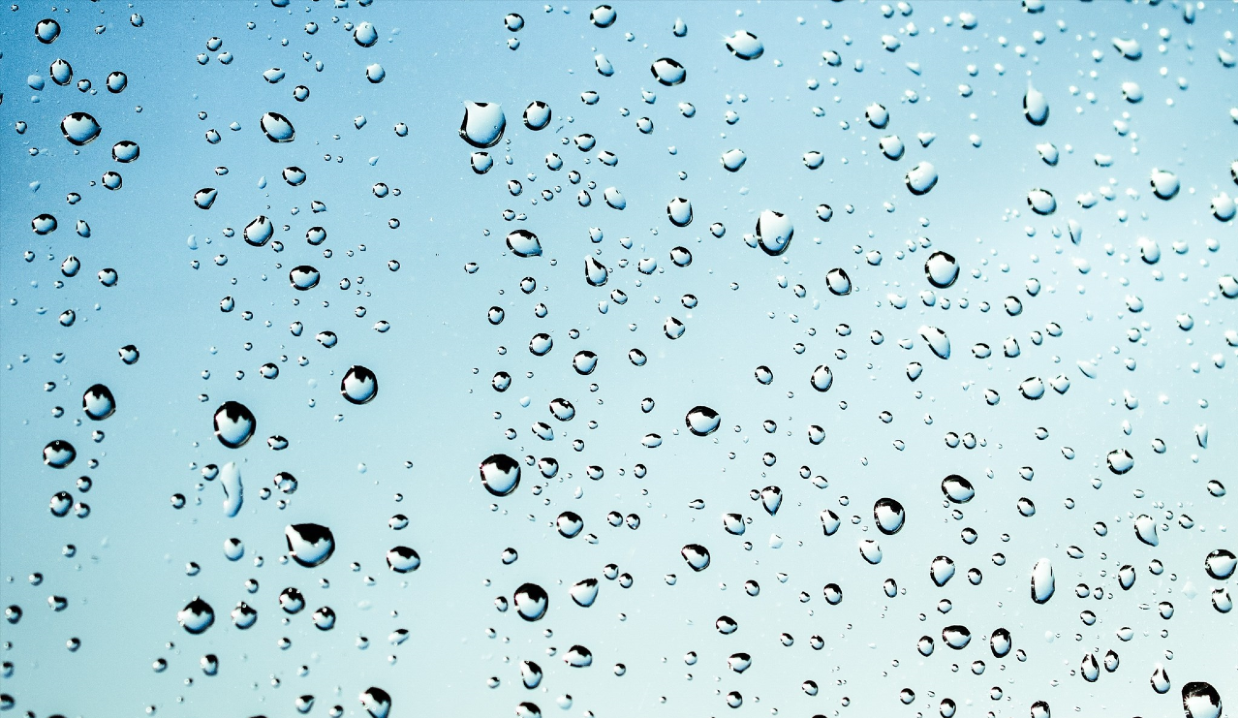
\includegraphics[width=\paperwidth]{Water3.png}};

\node[inner sep=0pt] (background) at (current page.north east) {
\includegraphics[scale=0.5, angle=-90]{BassettCTCLogo1.png}};
\node[inner sep=0pt] (background) at (8.1,-1) {
\includegraphics[scale=0.03, angle=0]{waterdrop.jpg}};

\draw (current page.center)node [fill=blue!1!white!10,fill opacity=.3,text opacity=1,inner sep=2cm]at (3,2){ \Huge\centering\bfseries\sffamily\parbox[c][][t]{\paperwidth}{\centering \textcolor{Bittersweet}{} \\\vspace{3cm}\textcolor{BurntOrange}{Drinking Water Treatment}\\[15pt] % Book title
% {\Large A Profound Subtitle}\\[20pt] % Subtitle
{}}}; % Author name
\end{tikzpicture}
%\begin{center}
%
\includegraphics[scale=1, angle=-90]{BassettCTCLogo1.png} 
%\end{center}












%\begin{tikzpicture}[]
%\path[help lines,step=.2] (0,0) grid (16,6);
%\path[help lines,line width=.6pt,step=1] (0,0) grid (16,6);
%
%\node[inner sep=0pt] (background) at (current page.center) {\includegraphics[width=\paperwidth]{WaterBackground1.png}};
%\draw (current page.center)node [fill=blue!1!white!10,fill opacity=.3,text opacity=1,inner sep=2cm] { \Huge\centering\bfseries\sffamily\parbox[c][][t]{\paperwidth}{\centering \textcolor{Bittersweet}{October 2022} \\\textcolor{BurntOrange}{Drinking Water Treatment}\\[15pt]
%
%  \pgftext{
\includegraphics[width=300pt, angle =-90]{BassettCTCLogo1.png}} at (16,5);
%%  \pgftext{\includegraphics[width=150pt]{pic2.png}} at (0,0);
%\end{tikzpicture}
\vfill
\endgroup

%----------------------------------------------------------------------------------------
%	COPYRIGHT PAGE
%----------------------------------------------------------------------------------------

\newpage
~\vfill
\thispagestyle{empty}

\noindent Copyright \copyright\ 2022 Shabbir Basrai\\ % Copyright notice
%
%\noindent \textsc{Published by Publisher}\\ % Publisher
%
%\noindent \textsc{book-website.com}\\ % URL
%
%\noindent Licensed under the Creative Commons Attribution-NonCommercial 3.0 Unported License (the ``License''). You may not use this file except in compliance with the License. You may obtain a copy of the License at \url{http://creativecommons.org/licenses/by-nc/3.0}. Unless required by applicable law or agreed to in writing, software distributed under the License is distributed on an \textsc{``as is'' basis, without warranties or conditions of any kind}, either express or implied. See the License for the specific language governing permissions and limitations under the License.\\ % License information, replace this with your own license (if any)

\noindent \textit{Revision Date: October 2022} % Printing/edition date

%----------------------------------------------------------------------------------------
%	TABLE OF CONTENTS
%----------------------------------------------------------------------------------------

%\usechapterimagefalse % If you don't want to include a chapter image, use this to toggle images off - it can be enabled later with \usechapterimagetrue

\chapterimage{WaterChapterImage} % Table of contents heading image

\pagestyle{empty} % Disable headers and footers for the following pages

\tableofcontents % Print the table of contents itself
\listoffigures
\listoftables
\cleardoublepage % Forces the first chapter to start on an odd page so it's on the right side of the book

\pagestyle{fancy} % Enable headers and footers again

%----------------------------------------------------------------------------------------
%	PART
%----------------------------------------------------------------------------------------



%----------------------------------------------------------------------------------------
%	CHAPTER 1
%----------------------------------------------------------------------------------------

% \chapterimage{chapter_head_2.pdf} % Chapter heading image

% \chapter{Text Chapter}

% \section{Paragraphs of Text}\index{Paragraphs of Text}



% \lipsum[1-7] % Dummy text
% 
%------------------------------------------------

%\section{Citation}\index{Citation}
%
%This statement requires citation \cite{article_key}; this one is more specific \cite[162]{book_key}.

%------------------------------------------------

%\section{Lists}\index{Lists}
%
%Lists are useful to present information in a concise and/or ordered way\footnote{Footnote example...}.
%
%\subsection{Numbered List}\index{Lists!Numbered List}
%
%\begin{enumerate}
%\item The first item
%\item The second item
%\item The third item
%\end{enumerate}
%
%\subsection{Bullet Points}\index{Lists!Bullet Points}
%
%\begin{itemize}
%\item The first item
%\item The second item
%\item The third item
%\end{itemize}
%
%\subsection{Descriptions and Definitions}\index{Lists!Descriptions and Definitions}
%
%\begin{description}
%\item[Name] Description
%\item[Word] Definition
%\item[Comment] Elaboration
%\end{description}


%----------------------------------------------------------------------------------------
%	PART 2
%----------------------------------------------------------------------------------------


%----------------------------------------------------------------------------------------
%	CHAPTER 1
%----------------------------------------------------------------------------------------

%\chapter{Wastewater Math}

\part{Module 1}
\chapterimage{WaterChapterImage1}
\chapter{Water Systems Operator Certifications}
\pagestyle{empty}
\newpage
\pagestyle{empty}
\begin{table}[H]
\captionsetup{justification=centering}
\scriptsize

%\tiny, \scriptsize, \footnotesize, \small, \normalsize, \large, \Large, \LARGE, \huge, and \Huge.
\begin{tabular}{|c|p{7.1cm}|p{7cm}|}
\hline
\thead{Grade} & \thead{Minimum Qualifications for\\ Examination                                                                                                                                                                                                                                                                                            } & \thead{Eligibility Criteria for\\ Certification                                                                                                                                                                                                                                                                                                                                                                                                                      } \\ \hline
D1    & High School Diploma / GED Equivalency*                                                                                                                                                                                                                                                                                             & \makecell[l]{Successful completion of the Grade   D1 examination within \\the three years prior to\\submitting certification application.                                                                                                                                                                                                                                                                                                                                 } \\ 
\hline
D2    & \makecell[l]{High School Diploma / GED Equivalency*\\ AND\\ One 3-unit (or 36-hour) course of specialized training covering\\the fundamentals of water supply principles.} & \makecell[l]{Successful completion of the Grade D2 examination within \\the three years prior to submitting certification \\application}.                                                                                                                                                                                                                                                                                                                                \\ 
\hline
D3    & \makecell[l]{Current D2 Certification\\AND\\Two 3-unit (or 36-hour) courses of specialized training that\\includes at least one course in the fundamentals of water supply\\ principles and a second course in either drinking water\\distribution, treatment, or   wastewater treatment.} & \makecell[l]{Successful completion of the Grade D3 examination within\\the three years prior to submitting certification application\\AND\\At least one year of operator experience working as a certified\\D2 operator for a D2 system or higher\\AND\\At least one additional year of operator experience working\\as a distribution operator. This may be substituted with (1)\\or (2) below.}\\ 
\hline
D4    & \makecell[l]{Current D3 certification\\ AND \\Three 3-unit (or 36-hour) courses of specialized training\\that includes at least two courses in the fundamentals of water supply\\ principles and a third course in either drinking water distribution,\\treatment, or wastewater treatment.}& \makecell[l]{Successful completion of the Grade   D4 examination within the \\three years prior to submitting the application for certification\\ AND\\ At least one year of operator experience working as a\\certified D3 operator for a D3 system or higher\\ AND\\ At least three additional years of operator experience working\\as a distribution operator. This may be substituted with (1)\\or (2) below.}\\ \hline
D5    & \makecell[l]{Current D4 certification\\AND\\Four 3-unit (or 36-hour) courses of specialized training\\ that includes at least two courses in the fundamentals of water\\supply principles and two additional courses in either\\ drinking water distribution, treatment, or wastewater treatment.} & \makecell[l]{Successful completion of the Grade D5 examination within\\the three years prior to submitting the application for\\certification\\AND\\At least two years of operator experience working as a\\certified D4 operator for a D4 or D5 system\\AND\\At least three additional years of operator experience\\working as a distribution operator. This may be substituted\\with (1) or (2) below.}\\ \hline
\end{tabular}

\footnotesize{\caption{Drinking Water Distribution\\
Minimum Qualifications for Examination and Eligibility Criteria for Certification}}

\end{table}
\begin{tiny}

High School Diploma/GED equivalency for Grades 1 and 2 ONLY can be fulfilled with either successful completion of Basic Small Water Systems Operations course provided by the Department OR 1 year as an operator of a facility that required an understanding of a piping system that included pumps, valves, and storage tanks.\\

"Experience substitutions for certification, as referenced above.
\begin{enumerate}[]
\item A relevant degree earned at an accredited academic institution may be substituted as follows:
\begin{enumerate}[label=(\alph*)]
\item Associate’s Degree or Certificate in Water or Wastewater Technology that includes at least 15 units of physical, chemical, or biological science may be used to fulfill 1 year of operator experience.
\item Bachelor’s Degree in engineering or in physical, chemical, or biological sciences (e.g. Biology, Chemical Engineering, Chemistry, Civil Engineering, Environmental Engineering, Microbiology, Public Health, or Sanitary Engineering) may be used to fulfill 1.5 years of operator experience.
\item Master’s Degree in the above mentioned fields in (b) may be used to fulfill 2 years of operator experience.
\end{enumerate}
\item A certified operator may substitute, on a day-for-day basis, 1 additional year of operator experience working as a distribution operator with experience gained while working with lead responsibility for water quality or quantity related projects or research."	
\end{enumerate}	
\end{tiny}

\newpage
\pagestyle{empty}
\begin{table}[H]
\captionsetup{justification=centering}
\scriptsize

\begin{tabular}{|c|p{7.1cm}|p{7cm}|}
\hline
\thead{Grade} & \thead{Minimum Qualifications for Examination                                                                                                                                                                                                                                                                                     } & \thead{Eligibility Criteria for Certification                                                                                                                                                                                                                                                                                                                                                                                                                                                                                                } \\
\hline
T1    & High School Diploma / GED Equivalency*.                                                                                                                                                                                                                                                                                     & Successful completion of the Grade   T1 examination within the three years prior to   submitting certification application.                                                                                                                                                                                                                                                                                                                                                                                                            \\
\hline
T2    & \makecell[l]{High School Diploma / GED Equivalency*\\AND\\One 3-unit (or 36-hour) course of specialized training covering\\the fundamentals of drinking water treatment.} & \makecell[l]{Successful completion of the Grade T2 examination within\\the three years prior to submitting certification application.                                                                                                                                                                                                                                                                                                                                                                                                           } \\
\hline
T3    & \makecell[l]{High School Diploma / GED Equivalency*\\AND\\Two 3-unit (or 36-hour) courses of specialized training\\that include at least one course in drinking water treatment and a \\second coursein either drinking water treatment, distribution,\\or wastewater treatment.}& \makecell[l]{Successful completion of the Grade T3 examination within the\\three years prior to   submitting certification application\\AND\\At least one year of operator experience working as a   certified\\T2 operator at a T2 facility or higher. This may be substituted\\with (3) below.\\AND\\      At least one additional year of operator experience working as a\\certified treatment operator. This may be substituted with\\(1), (2), or (4) below.}\\  
\hline                               
T4    & \makecell[l]{Current T3 certification\\AND\\Three 3-unit (or 36-hour) courses of specialized training that\\include at least two courses in the fundamentals of drinking\\water treatment and a third course in either\\drinking water treatment, distribution, or wastewater treatment.} & \makecell[l]{Successful completion of the Grade T4 examination within the\\three years prior to submitting the application\\for certification\\AND\\At least one year of operator experience working as shift\\or chief operator, while a certified T3 operator at a T3\\facility or   higher. This may be substituted with (3) below.\\AND\\At least three additional years of operator experience\\working as a certified treatment operator. This may be\\substituted with (1) or (4) below.}\\
\hline
T5    & \makecell[l]{Current T4 certification\\AND\\Four 3-unit (or 36-hour) courses of specialized training that\\include\\at least two courses in drinking water treatment and two \\additional   courses in either drinking water treatment, \\distribution,or wastewater   treatment.}              & \makecell[l]{Successful completion of the Grade T5 examination within the\\three years prior to   submitting the application for certification\\AND\\At least two years of operator experience working as a   shift or\\chief operator, while a certified T4 operator at a T4 facility or \\ higher. There are no substitutions.\\AND\\At least three additional years of operator experience working\\ as a  certified treatment operator. This may be substituted with\\(1) or (4) below.} \\ 
\hline      
\end{tabular}
\caption{Drinking Water Treatment\\
Minimum Qualifications for Examination and Eligibility Criteria for Certification}
\end{table}
\begin{tiny}
"*High School Diploma/GED equivalency for Grades 1 and 2 ONLY can be fulfilled with either successful completion of Basic Small Water Systems Operations course provided by the Department
OR 1 year as an operator of a facility that required an understanding of a chemical feeds, hydraulic systems, and pumps."\\			
"Experience substitutions for certification, as referenced above.
\begin{enumerate}
\item A relevant degree earned at an accredited academic institution may be substituted as follows:
\begin{enumerate}[label=\alph*)]
\item Associate’s Degree or Certificate in Water or Wastewater Technology that includes at least 15 units of physical, chemical, or biological science may be used to fulfill 1 year of operator experience.
\item Bachelor’s Degree in engineering or in physical, chemical, or biological sciences (e.g Biology, Chemical Engineering, Chemistry, Civil Engineering, Environmental Engineering, Microbiology, Public Health, or Sanitary Engineering) may be used to fulfill 1.5 years of operator experience.
\item Master’s Degree in the above mentioned fields in (b) may be used to fulfill 2 years of operator experience.
\end{enumerate}
\item A certified operator may substitute, on a day-for-day basis, experience gained while working with lead responsibility for water quality related projects of research (e.g. pilot plant).
\item If an applicant has a Bachelor’s or Master’s of Science degree, completion of a comprehensive operator training program, pursuant to Section 63800(h), may be substituted for the required experience.
\item Experience gained as a certified wastewater treatment operator may be used to substitute up to 2 years of the experience requirement. Wastewater treatment operator experience is credited on a two-for-one basis (i.e. 2 months in wastewater=1 month in drinking water)."			
\end{enumerate}
\end{tiny}
\newpage
\pagestyle{empty}

\begin{table}[H]
\captionsetup{justification=centering}
\scriptsize
\begin{tabular}{|l|p{6.5cm}|l|p{6.5cm}|}
\hline

\multicolumn{1}{|c|}{\thead{PATH}} & 
  \multicolumn{1}{|c|}{\thead{EXAMINATION EDUCATION REQUIREMENTS}} & &\multicolumn{1}{|c|}{\thead{CERTIFICATION QUALIFYING EXPERIENCE \\REQUIREMENTS}}\\\hline


%\thead{PATH} & \thead{EXAMINATION EDUCATION REQUIREMENTS}&     &\thead{CERTIFICATION QUALIFYING EXPERIENCE \\REQUIREMENTS}\\ \hline
GRADE I   &                                                                                                                                                                                                                                                                                               &     &                                                                                                 \\ \hline
1         & High  school  diploma or equivalent and 6 educational pts                                                                                                                                                                                                                          & and & 1 year of full-time qualifying experience                                   \\ \hline
GRADE II  &                                                                                                                                                                                                                                                                                               &     &                                                                                                 \\ \hline
1         & High  school  diploma    or  equivalent  and    9 educational pts                                                                                                                                                                                                                          & and & 18   months   of     full-time   qualifying   experience as a Grade I operator                  \\ \hline
2         & High  school  diploma    or  equivalent  and    12 educational pts                                                                                                                                                                                                                         & and & 2    years    of      full-time    qualifying   experience                                      \\ \hline
3         & \makecell[l]{Associate’s  degree,  a    higher  degree,  or  a minimum   of\\   60  college   semester   units, including a minimum of 15\\semester units of science courses                                                                                                                          } & and & 1     year     of       full-time     qualifying   experience                                   \\ \hline
GRADE III &                                                                                                                                                                                                                                                                                               &     &                                                                                                 \\ \hline
1         & High  school  diploma    or  equivalent  and    12 educational pts                                                                                                                                                                                                                         & and & 3    years    of      full-time    qualifying   experience as a Grade II operator               \\ \hline
2         & High  school  diploma    or  equivalent  and    18 educational pts                                                                                                                                                                                                                         & and & 4    years    of      full-time    qualifying   experience                                      \\ \hline
3         & \makecell[l]{Associate’s  degree  or    a  minimum   of     60 college semester\\ units,including a minimum of 15 semester units of\\science courses                                                                                                                                                      } & and & 2    years    of      full-time    qualifying   experience                                      \\ \hline
4         & \makecell[l]{Bachelor’s   degree   or     a   higher   degree, including a\\ minimum of 30 semester   units of science courses                                                                                                                                                                              } & and & 1     year     of       full-time     qualifying   experience                                   \\ \hline
GRADE IV  &                                                                                                                                                                                                                                                                                               &     &                                                                                                 \\ \hline
1         & High  school  diploma    or  equivalent  and    32 educational points                                                                                                                                                                                                                         & and & 6    years    of      full-time    qualifying   experience                                      \\ \hline
2         & \makecell[l]{Associate’s   degree   or     a  minimum   of     60 college semester \\units, including a minimum of 15 semester units of   science\\ courses                                                                                                                                                   } & and & 4    years    of      full-time    qualifying   experience                                      \\ \hline
3         & \makecell[l]{Bachelor’s   degree   or     a   higher   degree, including a minimum\\ of 30 semester   units of science courses                                                                                                                                                                              } & and & 3    years    of      full-time    qualifying   experience                                      \\ \hline
4         &\makecell[l]{ Valid  registration  as    a  chemical,  civil,\\or mechanical     engineer     issued     by the California  Board \\ for    Professional  Engineers and  Land    Surveyors  or  by\\ another  state, territory, or   Indian tribe                                                   } & and & 2    years    of      full-time    qualifying   experience                                      \\ \hline
GRADE V   &                                                                                                                                                                                                                                                                                               &     &                                                                                                 \\ \hline
1         & High  school  diploma    or  equivalent  and    48 educational points                                                                                                                                                                                                                         & and & 10      years      full-time      qualifying experience                                         \\ \hline
2         & \makecell[l]{Associate’s   degree   or     a  minimum   of     60 college semester \\units, including a minimum of 15 semester units of   science\\courses                                                                                                                                                   } & and & 6    years    of      full-time    qualifying   experience                                      \\ \hline
3         & Bachelor’s   degree   or     a   higher   degree, including a minimum of 30 semester   units of science courses                                                                                                                                                                               & and & 5    years    of      full-time    qualifying   experience                                      \\ \hline
4         & \makecell[l]{Valid  registration  as    a  chemical,  civil,    or mechanical\\ engineer issued by the California  Board  for    Professional\\  Engineers and Land    Surveyors or  by another  state,  a \\territory, or an Indian tribe} & and & 4    years    of      full-time    qualifying   experience                                      \\ \hline
\end{tabular}
\caption{Wastewater Operator License Requirements}
\end{table}

\newpage


\begin{table}[H]
\captionsetup{justification=centering}
\scriptsize
\begin{tabularx}{\textwidth}{| X | X |}
%{
%|>{\setlength\hsize{1.\hsize}\setlength\linewidth{\hsize}}X|
%>{\setlength\hsize{.5\hsize}\setlength\linewidth{\hsize}}X|
%>{\setlength\hsize{.01\hsize}\setlength\linewidth{\hsize}}X|}

\hline
\multicolumn{2}{|l|}{Grade 3}                                                                                                                                                                                                                                                                                                                                                                                                   \\
\hline
\begin{itemize}
\item Possess a current state issued Drinking Water Treatment Operator Certification or Wastewater Treatment Plant   Operator Certification, Grade III or higher                                                                                                                                                                                             
\end{itemize} & 
\begin{itemize}
\item Successful completion of AWTO Grade 3 Exam (AWT3TM)
\end{itemize} \\
\hline
\multicolumn{2}{|l|}{Grade 4}                                                                                                                                                                                                                                                                                                                                                                                                   \\
\hline
\begin{itemize}
\item Possess a current AWT3 certification
\item 2 years of   experience with one or more AWT processes (see Table 1). Retroactive   experience prior to AWT3 certification may be included 
\end{itemize}
& 
\begin{itemize}
\item Successful   completion of AWTO Grade 4 Exam (AWT4TM) 
\end{itemize}\\
\hline
\multicolumn{2}{|l|}{Grade 5}                                                                                                                                                                                                                                                                                                                                                                                                  \\
\hline
\begin{itemize} 
\item Possess a   current AWT4 certification 
\item 3 years of   experience to include 2 years of experience in at least one AWT process and 1   additional year with at least 2 AWT processes in a single treatment train   (see Table 1). Retroactive experience prior to AWT4 certification may be   included. 
\end{itemize}
&\begin{itemize}
\item Successful completion of AWTO Grade 5 Exam (AWT5TM)
\end{itemize}\\
\hline
\end{tabularx}

\caption{Advanced Water Treatment Certification Requirements}
\end{table}

%\part{Module 2}
%\input{Water Properties and Laboratory Analysis Slides}
%\part{Module 3}
%\input{Math1 Slides.tex}
%\part{Module 4}
%\input{Water Sources1 Slides.tex}
%\part{Module 5}
%\input{Water Regulations Revised1 Slides.tex}
%\part{Module 6}
%\input{Water Treatment1 Slides}
%\part{Module 7}
%\input{Water Disinfection Slides.tex}

\end{document}
